\documentclass{article}
\usepackage{ae,aecompl}
\usepackage{todonotes}
\usepackage{chngcntr}
\usepackage{tikz-cd}
\usepackage{graphicx}
\graphicspath{ {./images/}}
\usepackage[all,cmtip]{xy}
\usepackage{amsmath, amscd}
\usepackage{amsthm}
\usepackage{amssymb}
\usepackage{amsfonts}
\usepackage{bm}
\usepackage{qsymbols}
\usepackage{latexsym}
\usepackage{mathrsfs}
\usepackage{mathtools}
\usepackage{cite}
\usepackage{color}
\usepackage{url}
\usepackage{enumerate}
\usepackage{verbatim}
\usepackage[draft=false, colorlinks=true]{hyperref}
\usepackage{pdfpages}
\usepackage[margin=1.2in]{geometry}
\usepackage{IEEEtrantools}

\usepackage{fancyhdr}


\usepackage[nameinlink]{cleveref}


\DeclareMathOperator*{\ac}{accept}
\DeclareMathOperator*{\amax}{argmax}
\DeclareMathOperator*{\amin}{argmin}
\DeclareMathOperator*{\Aut}{Aut}
\newcommand {\al}{{\alpha}}
\newcommand {\abs}[1]{{\left\lvert#1\right\rvert}}
\newcommand {\A}{{\mathcal{A}}}
\newcommand {\AM}{{\mathrm{AM}}}
\newcommand {\AMp}{{\AM_{p}^{X}\!(\Ri_\w)}}
\newcommand {\B}{{\mathcal{B}}}
\DeclareMathOperator*{\Be}{Bern}
\newcommand {\Br}{{\dot{B}}}
\newcommand {\Ba}{{\mathfrak{B}}}
\newcommand {\C}{{\mathbb C}}
\newcommand {\ce}{\mathrm{c}}
\newcommand {\Ce}{\mathrm{C}}
\newcommand {\Cc}{\mathrm{C_{c}}}
\newcommand {\Ccinf}{\mathrm{C_{c}^{\infty}}}
\DeclareMathOperator{\cov}{Cov}
\DeclareMathOperator{\DEV}{DEV}
\newcommand {\Di}{{\mathbb D}}
\newcommand {\dom}{\mathrm{dom}}
\newcommand{\dist}{\stackrel{\mathrm{dist}}{=}}
\newcommand {\ud}{\mathrm{d}}
\newcommand {\ue}{\mathrm{e}}
\newcommand {\eps}{\varepsilon}
\newcommand {\veps}{\varepsilon}
\newcommand {\vrho}{{\varrho}}
\newcommand {\E}{{\mathbb{E}}}
\newcommand {\Ec}{{\mathcal{E}}}
\newcommand {\Ell}{L}
\newcommand {\Ellp}{{L_{p}[0,1]}}
\newcommand {\Ellpprime}{{L_{p'}([0,1])}}
\newcommand {\Ellq}{{L_{q}([0,1])}}
\newcommand {\Ellqprime}{{L_{q'}([0,1])}}
\newcommand {\Ellr}{L^{r}}
\newcommand {\Ellone}{{L_{1}([0,1])}}
\newcommand{\Elltwo}{{L_{2}([0,1])}}
\newcommand{\Ellinfty}{L^{\infty}}
\newcommand{\Ellinftyc}{L_{\mathrm{c}}^{\infty}}
\newcommand{\exb}[1]{\exp\left\{#1\right\}}
\DeclareMathOperator*{\Ext}{Ext}
\newcommand{\F}{{\mathcal{F}}}
\newcommand{\Fe}{{\mathbb{F}}}
\newcommand{\G}{{\mathcal{G}}}
\newcommand{\HF}{\mathcal{H}_{\text{FIO}}^{1}(\Rd)}
\newcommand{\Hr}{H}
\newcommand{\HT}{\mathcal{H}}
\newcommand{\ui}{\mathrm{i}}
\newcommand{\I}{{I}}
\newcommand{\J}{{\mathcal{J}}}
\newcommand{\id}{{\mathrm{id}}}
\newcommand{\iid}{\stackrel{\mathclap{\normalfont\mbox{iid}}}{\sim}}
\newcommand{\im}{{\text{im }}}
\newcommand{\ind}{{\perp\!\!\!\perp}}
\DeclareMathOperator*{\Int}{int}
\newcommand{\intx}{{\overline{\int_{X}}}}
\newcommand{\inte}{{\overline{\int_{\E}}}}
\newcommand{\la}{\lambda}
\newcommand{\rb}{\rangle}
\newcommand{\lb}{{\langle}}
\newcommand{\La}{\Lambda}
\newcommand{\calL}{{\mathcal{L}}}
\newcommand{\lp}{{\mathcal{L}}^{p}}
\newcommand{\lpo}{{\overline{\mathcal{L}}^{p}\!}}
\newcommand{\Lpo}{{\overline{\Ell}^{p}\!}}
\newcommand{\M}{{\mathbf{M}}}
\newcommand{\Ma}{{\mathcal{M}}}
\newcommand{\N}{{{\mathbb N}}}
\newcommand{\Na}{{{\mathcal{N}}}}
\newcommand{\norm}[1]{\left\|#1\right\|}
\newcommand{\normm}[1]{{\left\vert\kern-0.25ex\left\vert\kern-0.25ex\left\vert #1 
    \right\vert\kern-0.25ex\right\vert\kern-0.25ex\right\vert}}
\newcommand{\Om}{{{\Omega}}}
\newcommand{\one}{{{\bf 1}}}
\newcommand{\pic}{\text{Pic }}
\newcommand{\ph}{{\varphi}}
\newcommand{\Pa}{{\mathbb{P}}}
\newcommand{\Po}{{\mathcal{P}}}
\newcommand{\Q}{{\mathbb{Q}}}
\newcommand{\R}{{\mathbb R}}
\newcommand{\Rd}{{\mathbb{R}^{d}}}
\DeclareMathOperator{\rej}{reject }
\newcommand{\Rn}{{\mathbb{R}^{n}}}
\newcommand{\cR}{{\mathcal{R}}}
\newcommand{\Rad}{{\mathrm{Rad}}}
\newcommand{\ran}{{\mathrm{ran}}}
\newcommand{\Ri}{{\mathrm{R}}}
\newcommand{\supp}{{\mathrm{supp}}}
\newcommand{\Se}{\mathrm{S}}
\newcommand{\Sp}{S^{*}(\Rn)}
\newcommand{\St}{{\mathrm{St}}}
\newcommand{\Sw}{\mathcal{S}}
\newcommand{\T}{{\mathcal{T}}}
\newcommand{\ta}{{\theta}}
\newcommand{\Ta}{{\Theta}}
\newcommand{\topp}{\stackrel{p}{\to}}
\newcommand{\todd}{\stackrel{d}{\to}}
\newcommand{\toL}[1]{\stackrel{L^{#1}}{\to}} 
\newcommand{\toas}{\stackrel{a.s.}{\to}}
\DeclareMathOperator{\V}{Var}
\newcommand {\w}{{\omega}}
\newcommand {\W}{{\mathrm{W}}}
\newcommand {\Wnp}{\text{$\mathrm{W}$\textsuperscript{$n,\!p$}}}
\newcommand {\Wnpeq}{\text{$\mathrm{W}$\textsuperscript{$n\!,\!p$}}}
\newcommand {\Wonep}{\text{$\mathrm{W}$\textsuperscript{$1,\!p$}}}
\newcommand {\Wonepeq}{\text{$\mathrm{W}$\textsuperscript{$1\!,\!p$}}}
\newcommand {\X}{{\mathcal{X}}}
\newcommand {\Z}{{{\mathbb Z}}}
\newcommand {\Za}{{\mathcal{Z}}}
\newcommand {\Zd}{{\Z[\sqrt{d}]}}
\newcommand {\vanish}[1]{\relax}

\newcommand {\wh}{\widehat}
\newcommand {\wt}{\widetilde}
\newcommand {\red}{\color{red}}

% Distributions
\newcommand{\normal}{\mathsf{N}}
\newcommand{\poi}{\mathsf{Poisson}}
\newcommand{\bern}{\mathsf{Bernoulli}}
\newcommand{\bin}{\mathsf{Binomal}}
\newcommand{\multi}{\mathsf{Multinomial}}
\newcommand{\Exp}{\mathsf{Exp}}



% put your command and environment definitions here




% some theorem environments
% remove "[theorem]" if you do not want them to use the same number sequence


  \newtheorem{thrm}{Theorem}
  \newtheorem{lemma}{Lemma}
  \newtheorem{prop}{Proposition}
  \newtheorem{cor}{Corollary}

  \newtheorem{conj}{Conjecture}
  \renewcommand{\theconj}{\Alph{conj}}  % numbered A, B, C etc

  \theoremstyle{definition}
  \newtheorem{defn}{Definition}
  \newtheorem{ex}{Example}
  \newtheorem{exs}{Examples}
  \newtheorem{question}{Question}
  \newtheorem{remark}{Remark}
  \newtheorem{notn}{Notation}
  \newtheorem{exer}{Exercise}




\title{STATS305B -- Lecture 4}
\author{Jonathon Taylor\\ Scribed by Michael Howes}
\date{01/12/22}

\pagestyle{fancy}
\fancyhf{}
\rhead{STATS305B -- Lecture 4}
\lhead{01/12/22}
\rfoot{Page \thepage}

\begin{document}
\maketitle
\tableofcontents
\section{Inference on contingency tables}
\subsection{Secondary Analysis}
Last time we saw two statistics for testing the hypothesis $H_0 : \pi_{ij}=\pi_{i+}\pi_{+j}$. Suppose that we do indeed reject $H_0$, a natural question is why. We will see that both our test statistics can be decomposed and these can highlight which counts broke the independence hypothesis.
\subsection{Pearson's test}
One of the tests we discussed was Pearson's $\chi^2$-test of independence. This test has statistic,
\[X^2 = \sum_{ij} \frac{(N_{ij}-\wh{\la}_{ij})^2}{\wh{\la}_{ij}}, \]
where $\wh{\la}_{ij} = \frac{n_{i+}n_{+j}}{n_{++}} = n_{++}\wh{\pi}_{i+}\wh{\pi}_{+j}$ are the MLE estimates under $H_0$. This is a score statistic with asymptotic distribution $X^2 \sim \chi^2_{(I-1)(J-1)}$.  The quantities $e_{ij} = \frac{N_{ij}-\wh{\la}_{ij}}{\sqrt{\wh{\la}_ij}}$ are called \emph{Pearson's residuals}. Since,
\[X^2 = \sum_{ij} e_{ij}^2,\]
the term $e_{ij}$ can be interpreted as the evidence from cell $i,j$ against $H_0$. One can ask if $N_{ij} \stackrel{?}{\sim} \normal(0,1)$ under $H_0$. This is not true since otherwise we would expect $X^2$ to have $IJ$ degrees of freedom. The corrected residuals,
\[r_{ij} = \frac{N_{ij}-\wh{\la}_{ij}}{\sqrt{\wh{\la}_{ij}(1-\wh{\pi}_{i+})(1-\wh{\pi}_{+j})}}, \]
are asymptotically $\normal(0,1)$. Consider the following example,
\begin{center}
    \begin{tabular}{cc|cccccc}
        &&\multicolumn{6}{c}{Belief in god}\\
        &&1&2&3&4&5&6\\
        \hline 
        \multirow{3}{*}{Education level}&1&19& 8& 27& 8& 47& 236\\
        &2&23& 39& 88& 49& 179& 706\\
        &3&28& 48& 89& 19& 104& 293
    \end{tabular}
\end{center}
The Pearson statistic can be calculated in R using the function \texttt{chisq.test()}. For the above data the statistic is approximately 76 and the p-value is approximately $3\times 10^{-12}$. The package \texttt{vcd} has a function \texttt{mosaic()} that can be used to visualize the Pearson's residuals and the departure from independence. When applied to the above table, \texttt{mosaic()} returns the following
\begin{center}
    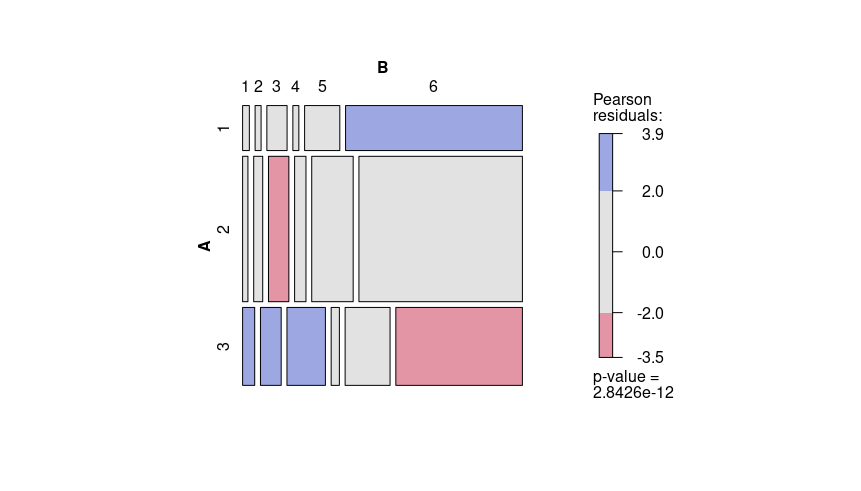
\includegraphics[width = \textwidth]{01_12_P01.jpg}
\end{center}
The area of each cell is proportional to the count in that cell. The rows have fixed width and the columns have variable widths. If $X$ and $Y$ were independent, then we would expect the columns to also have approximately the same width. Colored cells indicate cells with large Pearson's residuals with. Blue cells have a higher count than expected under independence and red cells have a lower count than under independence. It can be seen that there are more people with a high belief in god and a low education level than expected. Among people with a high level of education there are more than expected with a low belief in god and less than expected with a high belief in god.
\subsection{Likelihood ratio test}
Last lecture we also saw that we could test for independence with the statistic,
\[G^2 = -2\log(L_0) + 2\log(L_1),\]
where $L_0$ is the maximum likelihood under $H_0$ and $L_1$ is the maximum likelihood under $H_0 \cup H_1$ (we will sometimes say that $L_1$ is the maximum likelihood in the \emph{saturated model}). Under the null $H_0$, $G^2$ has asymptotic distribution $\chi^2_{(I-1)(J-1)}$. The statistic $G^2$ can also be calculated in R by using \texttt{lr\_stat()}. For the education level/belief in god table, we have $G^2 \approx 73 \approx X^2$ and a similar p-value to $X^2$.  We can also decompose $G^2$. Consider, the following data containing counts from schizophrenia patients.
\begin{center}
    \begin{tabular}{c|ccc}
       & biogenic & environmental & combination \\ 
        \hline
      eclectic & 90 & 12 & 78 \\ 
        medical & 13 & 1 & 6 \\ 
        psychoanalytic & 19 & 13 & 50
      \end{tabular}
\end{center}
This table has a likelihood ratio statistic of approximately 23. The degrees of freedom is 4 and thus this is a significant result. To decompose $G^2$ we must first define the sub-tables of an $I\times J$ table. For each $i,j$ such that $2 \le i \le I$ and $2 \le j \le J$, we can define a $2\times 2$ sub-table $T(i,j)$ as follows. We keep entry $(i,j)$, ignore entries with $h>i,k>j$ and marginalize the entries $(h,k)$ with $h < i$ or $j < k$. More precisely, if our original table had entries $n_{hk}$, then the entries of $T_{ij}$ are 
\[\begin{array}{c|c|c|}
    T(i,j)&1&2\\
    \hline 
    1&\sum_{h <i, k < j}n_{hk} & \sum_{h < i}n_{hj}\\
    \hline 
    2&\sum_{k < j} n_{ik} & n_{ij}\\
    \hline 
\end{array} \]
Thus $T(2,2)$ is the top-left $2\times 2$ table of our original $I\times J$ table. In general the table $T(i,j)$ contains the counts of $X < i, X=i$ against $Y <j,Y=j$. There are $(I-1)(J-1)$ such sub-tables. Each sub-table has a likelihood ratio statistic $G_{ij}^2 \sim \chi^2_1$. It turns out that 
\begin{equation}\label{decomp} G^2 = \sum_{2\le i \le I, 2\le j \le J} G_{ij}^2. \end{equation}
In the schizophrenia table this decomposition gives
\[G^2 \approx 23 = 0.3+1.4+13+8.3 \approx G_{2,2}^2+G_{2,3}^2+G_{3,2}^2+G_{3,3}^2. \]
So the main contribution to $G^2$ comes from $G_{3,2}^2$ and $G_{3,3}^2$.  The decomposition \eqref{decomp} holds because the terms in the decomposition are the result of comparing a simpler model to a more complex model (this will be explained later). In later terms, the more complicated models become the simpler models and so there is cancellation between the terms. This is because when comparing a model $M_r$ to the simpler model $M_s$, the corresponding term is of the form
\[\DEV(M_s)-\DEV(M_r),\]
where $\DEV(M)$ is the deviance of the model $M$ and is analogous to the sum of squared errors from the linear model. Thus, when comparing the most complicated model $M_k$ to the simplest model $M_0$, we can write the comparison as sequence of comparisons $M_0$ against $M_1$, $M_1$ against $M_2$, \ldots, $M_{k-1}$ against $M_k$. This is analogous to the ANOVA decomposition for linear models.
\subsection{Fisher's exact test}
Another way to do inference on $2 \times 2$ tables is to use Fisher's exact test. Suppose we use either the Poisson or multinomial model for our cell counts and consider the null $H_0 : \pi_{ij} = \pi_{i+}\pi_{+j}$. Under $H_0$, the marginals $N_{1+}, N_{2+}, N_{+1}, N_{+2}$ are sufficient statistics. Furthermore, given the marginals, the individual cell counts are determined by $N_{11}$ and 
\[N_{11}|N_{1+}, N_{2+}, N_{+1}, N_{+2} \sim \hyper(N_{+1}, N_{+2}, N_{1+}), \]
where $\hyper(a,b,k)$ described the distribution of the number of red balls when drawing $k$ balls without replacement from an urn with $a$ red balls and $b$ blue balls. The reason why $N_{11}$ follows the above distribution conditioned on the marginals is that we can think of drawing $N_{1+}$ 1's and 2's from an under with $N_{+1}$ 1's and $N_{+2}$ 2's. The number of 1's in such a draw is the value of $N_{11}$. Since we know the exact distribution of $N_{11}$ under the null, we can calculate exact p-values by using the hyper-geometric distribution.

This form of exact test can generalize to $I \times J$ tables, but it gets complicated. This is because conditioned on the marginals there are $(I-1)\times(J-1)$ free parameters for the entries $N_{ij}$. Understanding the distribution of these entries is tricky are requires clever sampling techniques. In particular, naive MCMC does not work.
\subsection{Ordinal Association}
In the last lecture we discussed Kruskal's $\gamma$. Recall that if are variables $X$ and $Y$ are ordinal, then we can define the parameter $\gamma = \frac{\pi_c-\pi_d}{\pi_c+\pi_d}$ where
\[\pi_c =2\sum_{ij}\pi_{ij} \sum_{h>i,k>j}\pi_{hk}, ~~\text{ and }~~\pi_d =2\sum_{ij}\pi_{ij} \sum_{h>i,k<j}\pi_{hk}. \]
The parameter $\gamma \in [-1,1]$ measures the ordinal association between $X$ and $Y$ with $\gamma = 0$ corresponding to no association, $\gamma > 0$ corresponding to positive association and $\gamma < 0$ corresponding to negative association. We also defined the estimator
\[\wh{\gamma} = \frac{C-D}{C+D}, \]
where
\[C = 2\sum_{ij}n_{ij} \sum_{h>i,k>j}n_{hk} ~~\text{ and }~~ D = 2\sum_{ij}n_{ij} \sum_{h > i, k<j} n_{hk}.  \]
But we are yet to study the variance of $\wh{\gamma}$. The variance of $\wh{\gamma}$ can be approximated by using the bootstrap. To do this we need to create bootstrap resamples of our contingency table, and it isn't clear how to do this. One strategy is to ``flatten'' our contingency table.
\begin{enumerate}
    \item We first create a new table with $n_{++}$ rows and 2 columns labelled $X$ and $Y$. Each row corresponds to an individual from our population. In each individual's row we record their $X$ and $Y$. We can indeed construct such a table from the contingency table since the contingency table records how many individuals have $X=i$ and $Y=j$.
    \item For $b=1,\ldots,B$, we then draw $n_{++}$ rows with replacement from the flattened table. From these we can calculate a contingency table $T_b$, and we can calculate the estimate $\wh{\gamma}^*b$.
    \item We can then use the sample $\wh{\gamma}^*_b$ to estimate the variance and quantiles of $\wh{\gamma}$. These can then be used to make confidence intervals. 
\end{enumerate}
Another way to measure ordinal association is to assign numerical values to the labels of $X$ and $Y$ and then perform linear regression of $Y$ onto $X$. This gives us an F-statistic that measures the linear relationship between $X$ and $Y$. Unfortunately the value of the F-statistic depends on the numerical values assigned to $X$ and $Y$, and there is no set rule for how to assign such values.
\section{Modelling binary data}
We now consider modelling binary data. Suppose that we have a model $(X_i,Y_i)_{i=1}^n$ where $Y_i \in \{0,1\}$, $X_i \in \R^p$ and $(X_i,Y_i)$ are i.i.d. Such data can appear in a variety of applications. For example,
\begin{itemize}
    \item Medical: presence/absence of a disease.
    \item Industrial: passes/fails a quality control test.
    \item Political: voter/non-voter.
\end{itemize}
Since $Y_i \in \{0,1\}$, the distribution of $Y|X$ is described by a single parameter
\[\pi(x) = \Pa(Y =1|X=x). \]
The negative log-likelihood is thus,
\[-\log L(\pi|Y) = \sum_{i=1}^n - Y_i \log\left(\frac{\pi_i}{1-\pi_i}\right)-\log(1-\pi_i).\]
Note that we are only modelling $Y$ in our likelihood. This corresponds to either a fixed design for $X$ or to having conditioned on $X$. The quantity $\log\left(\frac{\pi_i}{1-\pi_i}\right)$ is the \emph{log-odds} of $Y_i=1$. The function $\pi \mapsto \log\left(\frac{\pi}{1-\pi}\right)$ is called the logit function. It is an increasing function with domain $(0,1)$ and range $\R$. The inversion function is $F_{\text{logistic}}(\eta) = \frac{e^\eta}{1+e^{\eta}}$. The function $F_{\text{logistic}}$ is sigmoidal and is the CDF of the sigmoidal distribution.
\subsection{Logistic regression}
Define $\eta_i = \log\left(\frac{\pi_i}{1-\pi_i}\right)$. The negative log likelihood function in terms of $\eta_i$ is
\[-\log L(\eta|Y) = \sum_{i=1}^n -Y_i\eta_i +\log(1+e^{\eta_i}). \]
In \emph{logistic regression} we introduce the constraint $\eta_i = X_i^T\beta$. Thus 
\[-\log L(\beta|Y) = \sum_{i=1}^n -Y_iX_i^T\beta +\sum_{i=1}^n \log(1+\exp(X_i^T\beta)) = -(X\beta)^TY +\sum_{i=1}^n \log(1+\exp(X_i^T\beta)), \]
where $X \in \R^{n \times p}$ has rows $X_i^T$. We will see that this function is convex in $\beta$ and thus optimizing the negative log likelihood is tractable. It also means that we can add convex regularization or convex constraints to $\beta$ and we will still have a convex problem.  This is the default model in most software GLM models for binary data. 

To see that the function 
\[-\log L(\beta|Y)  = -(X\beta)^TY +\sum_{i=1}^n \log(1+\exp(X_i^T\beta)),\]
is indeed convex, note that it suffices to prove that $-\log L(\eta |Y)$ since the composition of a linear function followed by a convex function is convex. Note that we can write
\[-\log L(\eta|Y) = \sum_{i=1}^n \Lambda_B(\eta_i)-\eta_i Y_i, \]
where $\Lambda_B(\eta)$ is the CGF of the Bernoulli distribution. Namely, for an exponential family with natural parameters $\eta$ and sufficient statistics $W$, we have
\[\exp(\La(\eta)) = \E_0[\exp(\eta^T W)], \]
where the expectation is taken at $\eta = 0$. The function $\eta \mapsto \La(\eta)$ is convex for any exponential family which can be seen by taking derivatives or by applying H\"older's inequality. Thus, $-\log L(\eta|Y)$ and hence $-\log L(\eta|Y)$ are both convex.
\subsection{Interpretation of coefficients}
Note that if $\eta = X^T \beta$, then 
\[OR_{X_j} = \frac{ODDS(Y=1|\ldots, X_j = x_j+1,\ldots)}{ODDS(Y=1|\ldots, X_j = x_j,\ldots)} = e^{\beta_j}. \]
Thus, $\beta_j$ determines the change in the odds of success if $X_j$ increases by 1 and all other covariates are fixed. Note that $e^{\beta_j}$ is the odds ratio when $X_j$ increases by 1. The quantity $e^{\beta_j}$ does not tell us the relative risk 
\[RR_{X_j} =\frac{\Pa(Y=1|\ldots, X_j = x_j+1,\ldots)}{\Pa(Y=1|\ldots, X_j = x_j,\ldots)}. \]
However, we have seen that if $\Pa(Y=1|X=x)$ is small for all values of $x$, then $OR \approx RR$. Thus, under the rare disease hypothesis,
\[RR_{X_j} \approx OR_{X_j} = e^{\beta_j}.\]
\subsection{Other binary models}
Suppose there exists a quantity $T_i$ such that $T_i | X_i \sim F$ and 
\[Y_i = \begin{cases}
    1 & \text{if } T_i \le X_i^T \beta,\\
    0 & \text{if } T_i > X_i^T\beta.
\end{cases} \]
In this case $\Pa(Y_i = 1|X_i) = \Pa(T_i \le X_i^T\beta |X_i) = F(X_i^T\beta)$. If we set $\eta_i = \text{logit}(F(X_i^T\beta))$ where $\text{logit}(\pi) =\log\left(\frac{\pi}{1-\pi}\right)$, then our log-likelihood is 
\[-\log(\beta|Y) = \sum_{i=1}^n Y_i \text{logit}F(X_i^T\beta)-\log(1-F(X_i^T\beta)).\]
Unfortunately, there is no guarantee that this will be convex in $\beta$. However, for the natural choice of $F = \Phi$ the CDF of $\normal(0,1)$, then this is convex and this model is called the \emph{probit model}. The parameters $\beta_j$ are not as interpretable in this type of model.
\subsection{Over dispersion}
One last comment is that for binary data we have
\[\V(Y) = \pi(1-\pi) = \E[Y](1-\E[Y]). \]
Thus, the expectation of $Y$ determines the variance of $Y$ (and indeed all higher moments).  This relates to the fact that logistic regression is a generalized linear model, and it relates to a concept called \emph{over-dispersion}.
\end{document}